\chapter{Development}
\section{Considerations}
\subsection{Xcorr}
\subsubsection{Theory}
Cross-correlation is a method used for comparing two signals. This can for example be with the purpose of finding specific features, patterns or identical signals.


\begin{equation}
\label{eq:xcross}
\centering
(f\star g)(t)=\sum\limits_{m=-\infty}^{m=\infty}f(t)*g(t+m)
\end{equation}
The equation in \ref{eq:xcross} is the mathematical expression of cross-correlation of discrete functions.

In figure \ref{fig:xcrossSample} two signals are present. We can use cross-correlation to find out how much these two signals are similar. This can be done using equation \ref{eq:xcross}. Since our signal doesn't go to $\infty$, but only to 7, we will let $m=-7$ to $m=7$, so our equation will be the one shown in \ref{eq:xcross2}.

\begin{equation}
\label{eq:xcross2}
\centering
(f\star g)(t)=\sum\limits_{m=-7}^{m=7}f(t)*g(t+m)
\end{equation}

We can establish from the graph that the two signals have consist of the two following data sets:
Green: \[0,1,2,1,0,0,0\]
Blue: \[0,0,0,1,2,1,0\]
These are the data points from 1-7. Any data point outside of that range will be zero. We will also use $t=-7$ to $t=7$ to cover the negative side in case of a left side shift.

We can then, following equation \ref{eq:xcross2}, calculate the cross-correlation:

\begin{center}
$(f\star g)(-7)=f(-7)*g(-7+(-7)+f(-7)*g(1+(-6))+...+f(-7)*g(-7+6)+f(1)*g(-7+7)$\\
$(f\star g)(-6)=f(-6)*g(-6+(-7)+f(-6)*g(2+(-6))+...+f(-6)*g(-6+6)+f(2)*g(-6+7)$\\
$(f\star g)(-5)=f(-5)*g(-5+(-7)+f(-5)*g(3+(-6))+...+f(-5)*g(-5+6)+f(3)*g(-5+7)$\\
$...$\\
$(f\star g)(0)=f(0)*g(0+(-7)+f(0)*g(0+(-6))+...+f(0)*g(0+6)+f(0)*g(0+7)$\\
$(f\star g)(1)=f(1)*g(1+(-7)+f(1)*g(1+(-6))+...+f(1)*g(1+6)+f(1)*g(1+7)$\\
$(f\star g)(2)=f(2)*g(2+(-7)+f(2)*g(2+(-6))+...+f(2)*g(2+6)+f(2)*g(2+7)$\\
$...$\\
$(f\star g)(6)=f(6)*g(6+(-7)+f(6)*g(6+(-6))+...+f(6)*g(2+6)+f(6)*g(6+7)$\\
$(f\star g)(7)=f(7)*g(7+(-7)+f(7)*g(7+(-6))+...+f(7)*g(3+6)+f(7)*g(7+7)$\\
\ \\
$(f\star g)(-7)=0$\\
$(f\star g)(-6)=0$\\
$(f\star g)(-5)=0$\\
$(f\star g)(-4)=0$\\
$(f\star g)(-3)=0$\\
$(f\star g)(-2)=0$\\
$(f\star g)(-1)=0$\\
$(f\star g)(0)=1$\\
$(f\star g)(1)=4$\\
$(f\star g)(2)=6$\\
$(f\star g)(3)=4$\\
$(f\star g)(4)=1$\\
$(f\star g)(5)=0$\\
$(f\star g)(6)=0$\\
$(f\star g)(7)=0$\\
\end{center}

Instead of letting m be in the range of $-\infty$ to $\infty$, we will let our sample size control the range, as in equation \ref{eq:xcrossN}
\begin{equation}
\label{eq:xcrossN}
\centering
(f\star g)(t)=\sum\limits_{m=-N}^{m=N}f(t)*g(t+m)
\end{equation}


\subsubsection{Test Matlab}
Before we went any further with the project we investigated which kind of signals which was good to send. We did that by generating a signal, made a delay and then cross-correlated these two signals, chirp, sinusoid and noise.
We tried three different signals\\
\textbf{Chirp}:\\
We started with a chirp. We did that because of gut feeling. We thought this would be the best signal to send mostly because it was controlled and not random, and the signal changed characteristic over time.\\
Below is shown the code we used to generate the signal, make the delay and do the cross-correlation:
\begin{lstlisting}[language=Matlab,frame=lrtb,label=Matlab Code for Chirp Cross-correlation]
Fs=48000;                                       % Sample frequency
t = [0:1/Fs:1];                                % Timeinterval and length
Frq1=14000;                                     % Start frequency for chirp
Frq2=14100;                                     % End frequency for chirp
delay = 2000;                                   % Signal Delay
Chirp_signal=chirp(t,Frq1,1,Frq2);              % Chirp signal generation
Chirp_delayed=[zeros(1,delay) Chirp_signal];    % Chip delay generation
Chirp_xcorr=xcorr(Chirp_signal,Chirp_delayed);  % Cross-correlation
LengthChirp_xcorr=length(Chirp_xcorr)           % Calculate length of Xcorr
[XmaxChirp_xcorr,YmaxChirp_xcorr]=max(Chirp_xcorr) % Find maximum value
Delay_calcX1X2=((LengthChirp_xcorr+1)/2)-YmaxChirp_xcorr % Calculate Delay
\end{lstlisting}
Below is the plot of the cross-correlation. It shows clearly where the to signal overlap.\\
\begin{figure}[H]
\centering
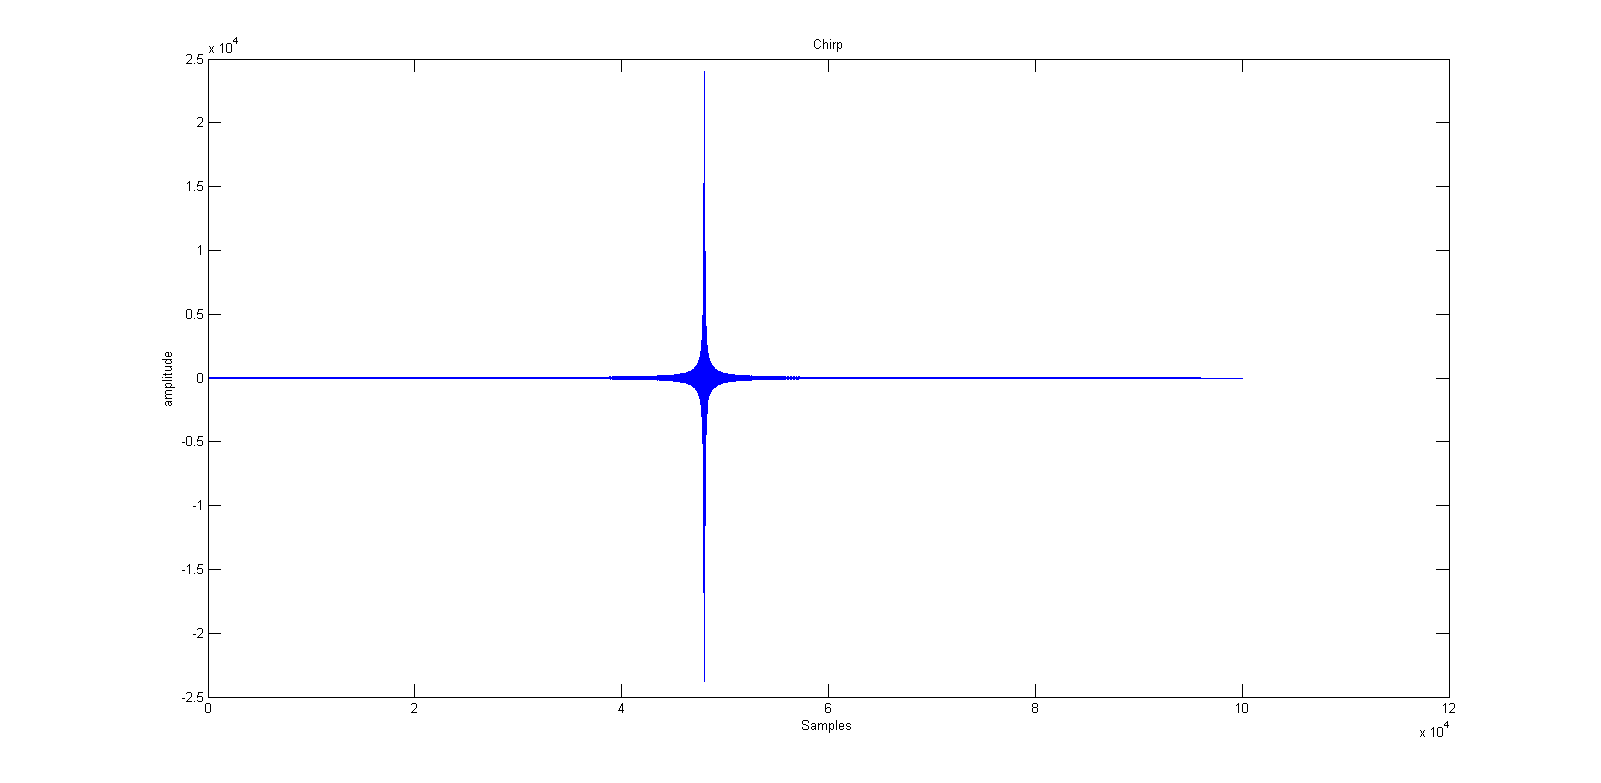
\includegraphics[width=0.6\textwidth]{billeder/chirp_xcorr_fig}
\caption{Plot of Cross-correlation of chirp signals}
\label{fig:chirp_xcorr_plot}
\end{figure}
The figure clearly shows where the two signals perfectly overlap. So the chirp seems like a good signal to use. although it isn't perfectly sharp in one sample it is quite distinct.\\
\textbf{Sinusoid}:\\
Similar code as the chirp was used to make two sinusoid signal. Below is a plot of a 14kHz sinus delayed with the same amount as the chrip signal.\\
\begin{figure}[H]
\centering
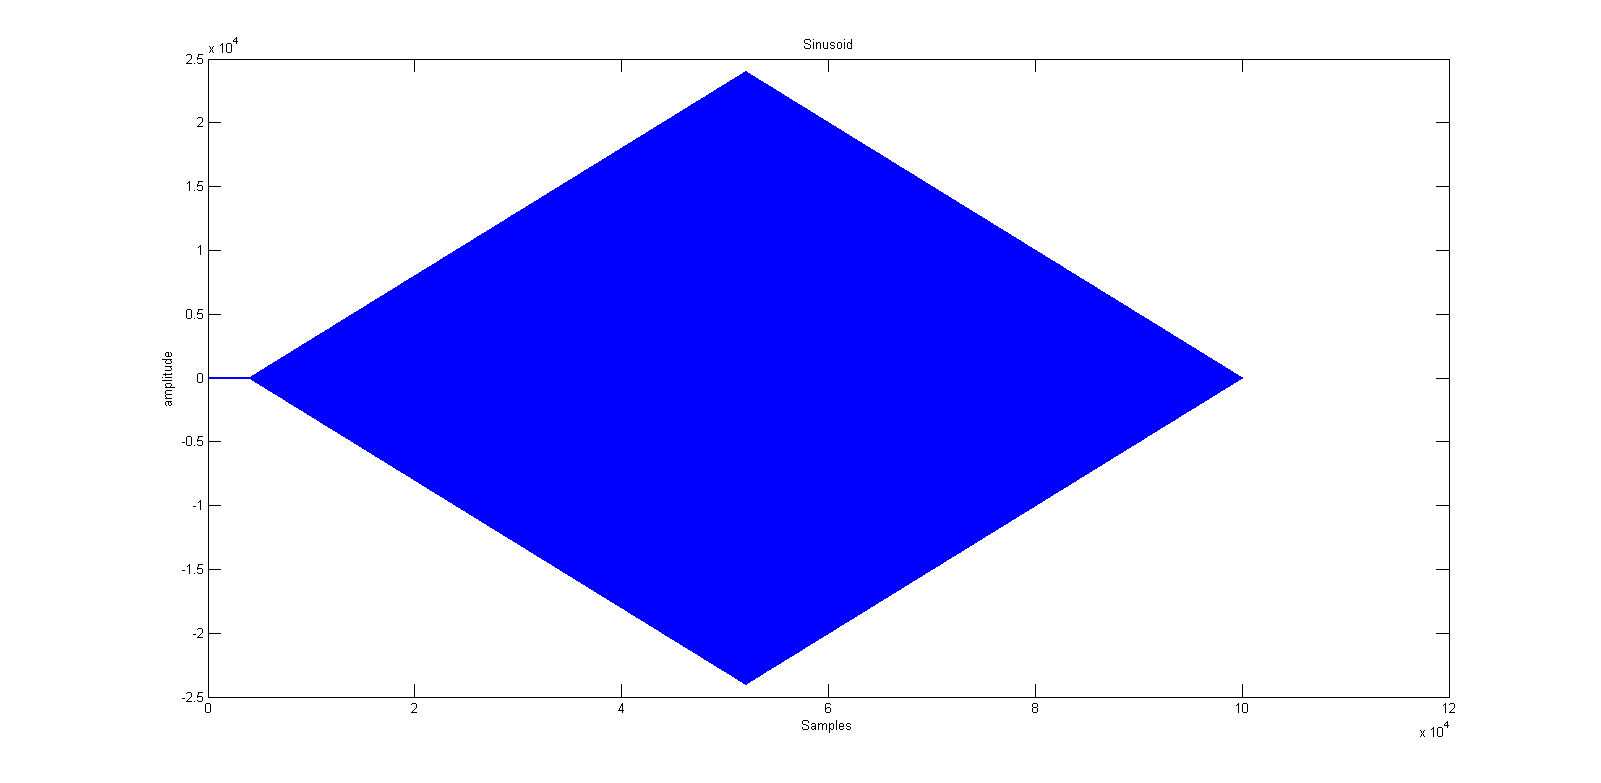
\includegraphics[width=0.6\textwidth]{billeder/sinus_xcorr_fig}
\caption{Plot of Cross-correlation of sinusoid signal}
\label{fig:sinus_xcorr_plot}
\end{figure}
This cross-correlation doesnt have as nice a peak as the chirp did and therefore we discarded using a sinusoid. The correlation looks like this because the sinus will make a spike every period because the periods will overlay eachother, this will increase until the signals completely overlays eachother.\\
\textbf{Noise}:\\
Lastly we tried generating a noise signal using the built-in function wgn (white gaussian noise). Below is shown the cross-correlation of the noise signals.\\
\begin{figure}[H]
\centering
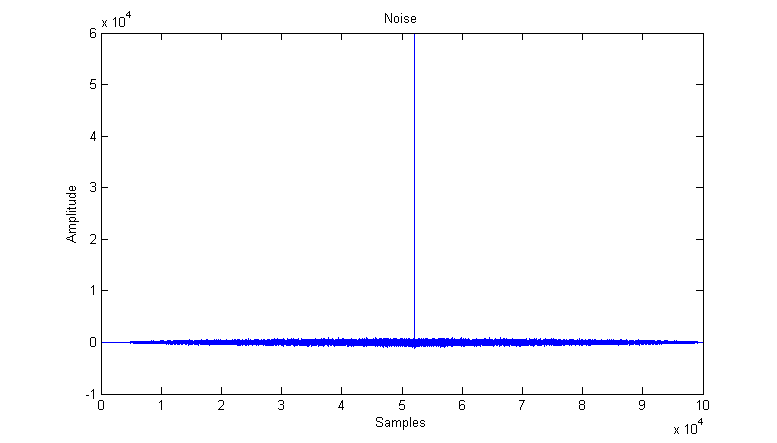
\includegraphics[width=0.6\textwidth]{billeder/noise_xcorr_fig}
\caption{Plot of cross-correlation of noise signal}
\label{fig:noise_xcorr_plot}
\end{figure}
This correlation made an even harder spike then the chirp. This is because of the fact that the  two noise signal only are similar in a very specific point. When they are not completely overlaying each other most samples end up cancelling each others.
\subsection{Findings based on examination in matlab}
It is clear that the chirp as well as the noise are very distinct peaks where the signals overlap. 
